\begin{figure}[!ht]
\centering
\resizebox{\linewidth}{!}{
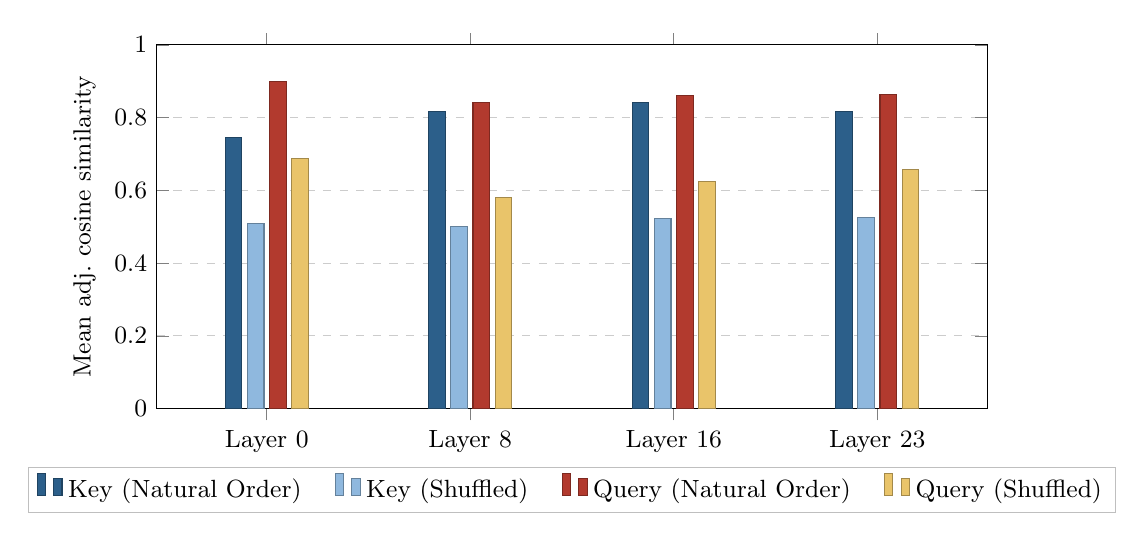
\begin{tikzpicture}
  \definecolor{keyReal}{HTML}{2C5F8A}   % dark blue
  \definecolor{keyShuf}{HTML}{8FB8DE}   % light blue
  \definecolor{queryReal}{HTML}{B23A2E} % dark red
  \definecolor{queryShuf}{HTML}{E9C46A} % light amber
  \begin{axis}[
    ybar,
    bar width=6pt,
    width=\textwidth,
    height=6.2cm,
    enlarge x limits=0.18,
    ymin=0, ymax=1,
    ytick={0,0.2,0.4,0.6,0.8,1.0},
    ylabel={Mean adj.\ cosine similarity},
    symbolic x coords={Layer 0, Layer 8, Layer 16, Layer 23},
    xtick=data,
    tick label style={font=\small},
    ylabel style={font=\small},
    ymajorgrids=true,
    grid style={dashed, gray!40},
    legend style={
      at={(0.5,-0.16)}, anchor=north,
      legend columns=4, font=\small,
      /tikz/every even column/.append style={column sep=10pt},
      draw=gray!50,
    },
  ]
    \addplot[fill=keyReal,   draw=keyReal!70!black]   coordinates {(Layer 0,0.7457) (Layer 8,0.8167) (Layer 16,0.8423) (Layer 23,0.8172)};
    \addplot[fill=keyShuf,   draw=keyShuf!70!black]   coordinates {(Layer 0,0.5094) (Layer 8,0.5005) (Layer 16,0.5216) (Layer 23,0.5242)};
    \addplot[fill=queryReal, draw=queryReal!70!black] coordinates {(Layer 0,0.9000) (Layer 8,0.8408) (Layer 16,0.8619) (Layer 23,0.8626)};
    \addplot[fill=queryShuf, draw=queryShuf!70!black] coordinates {(Layer 0,0.6880) (Layer 8,0.5807) (Layer 16,0.6234) (Layer 23,0.6570)};
    \legend{Key (Natural Order), Key (Shuffled), Query (Natural Order), Query (Shuffled)}
  \end{axis}
\end{tikzpicture}
}
\caption{Average cosine similarity of adjacent key and query states for LLaMA-3.1 8B Instruct, showing both natural token order (post-RoPE) and randomly shuffled token order.}
\label{fig:combined_similarity}
\end{figure}
